\documentclass{standalone}
\usepackage{tikz}
\usetikzlibrary{patterns, positioning}
\usepackage[sfdefault]{ClearSans} %% option 'sfdefault' activates Clear Sans as the default text font
\usepackage[T1]{fontenc}

\begin{document}
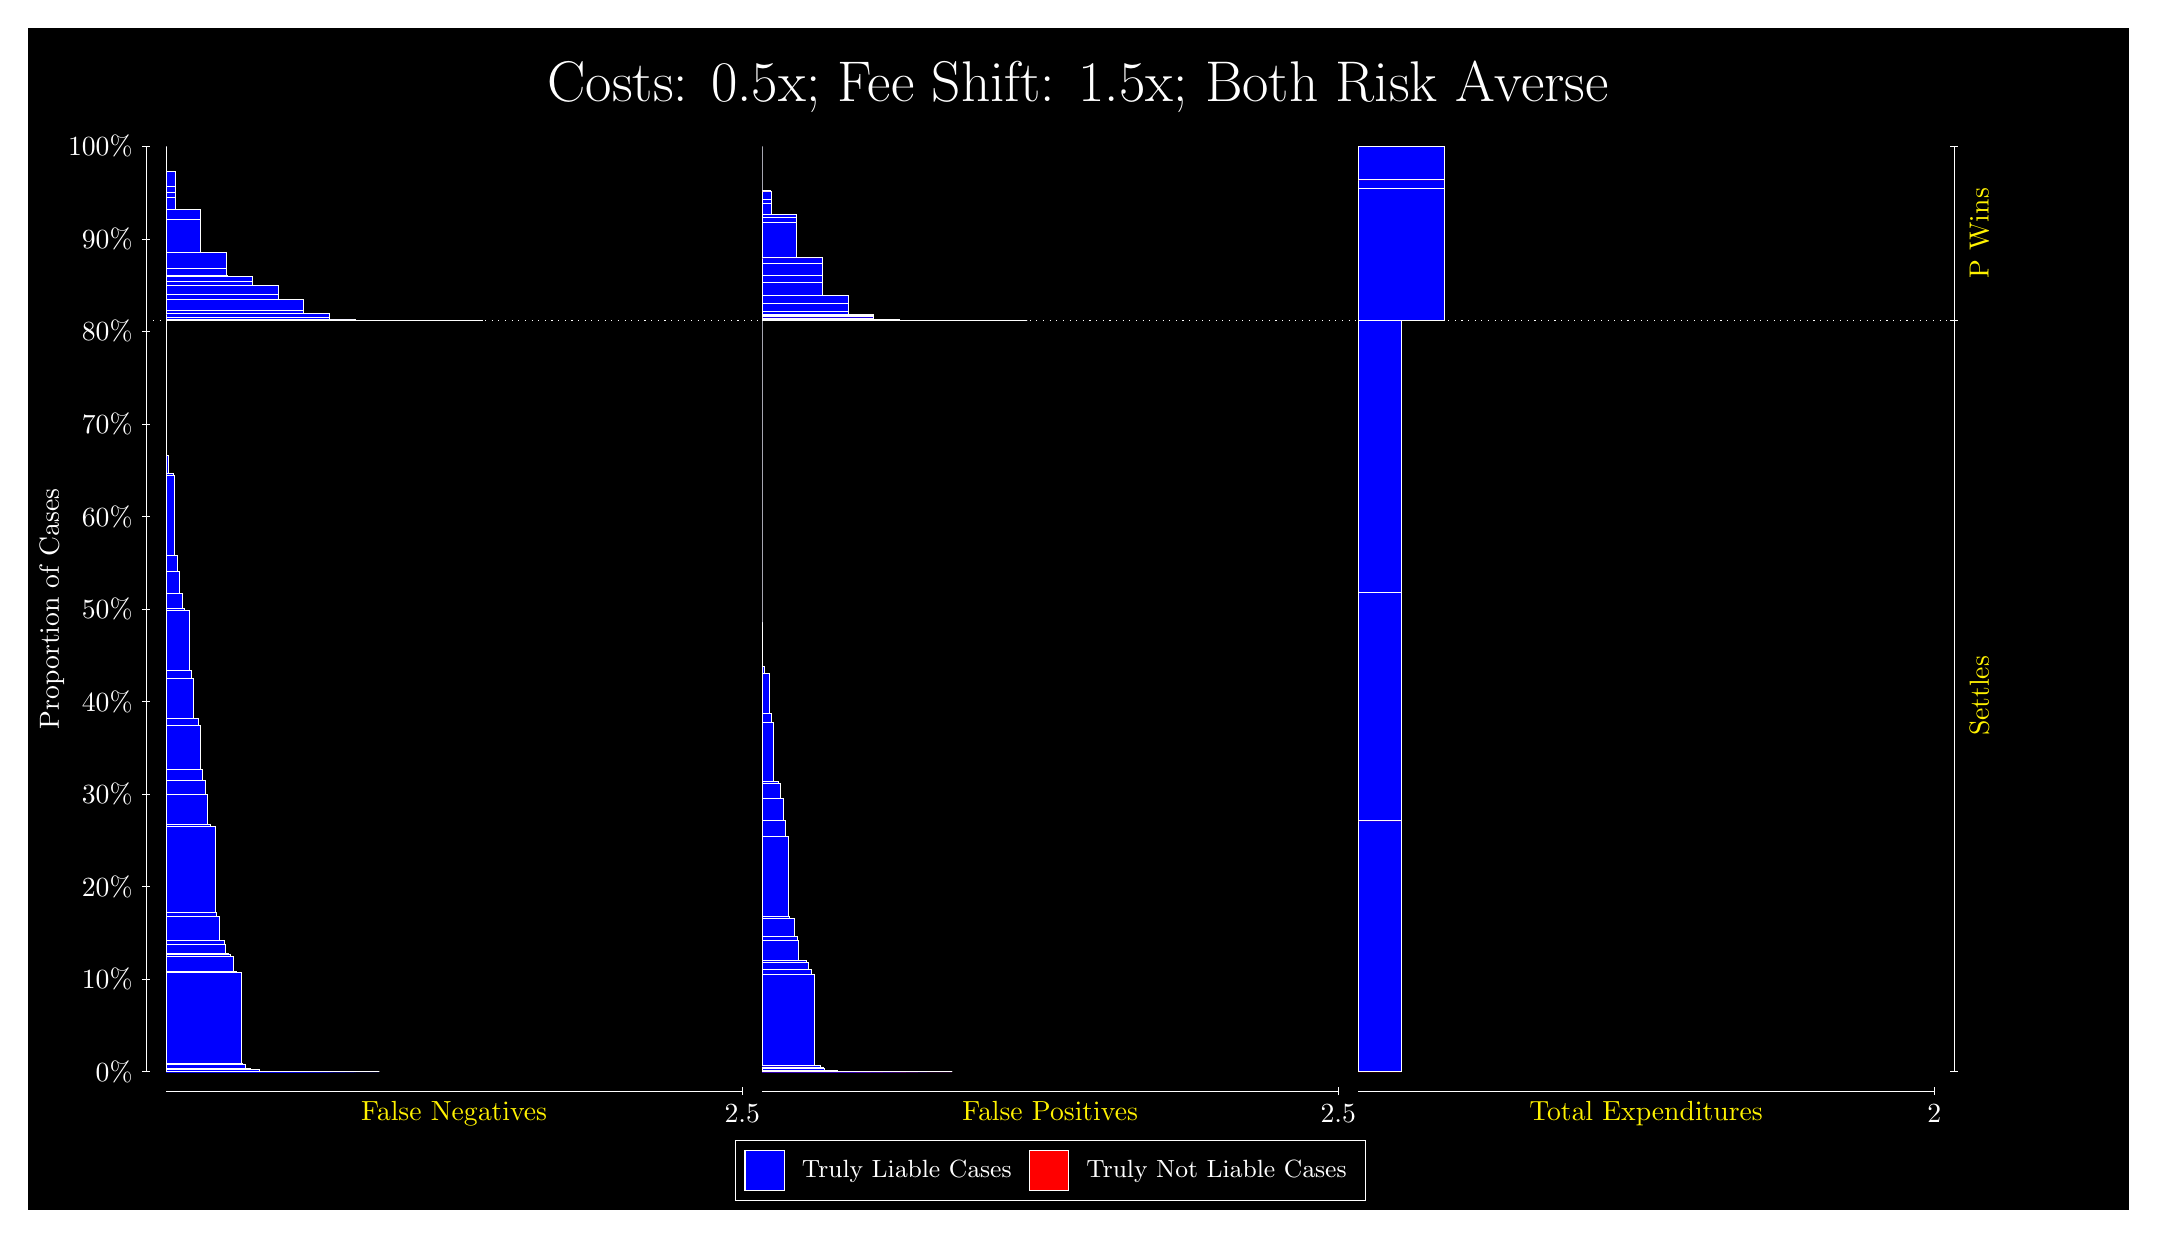
\begin{tikzpicture}
\draw[fill=black] (0,0) rectangle (26.667,15);
\draw[text=white] (0,13.5) rectangle (26.667,15) node[midway] {\huge Costs: 0.5x; Fee Shift: 1.5x; Both Risk Averse};
\draw[white, very thin] (1.5,1.75) -- (1.5,13.5);
\node[rotate=90, text=white, anchor=center] at (0.3, 7.625) {Proportion of Cases};
\draw[white, very thin] (1.45,1.75) -- (1.55,1.75);
\node[text=white, anchor=east] at (1.45, 1.75) {0\%};
\draw[white, very thin] (1.45,2.925) -- (1.55,2.925);
\node[text=white, anchor=east] at (1.45, 2.925) {10\%};
\draw[white, very thin] (1.45,4.1) -- (1.55,4.1);
\node[text=white, anchor=east] at (1.45, 4.1) {20\%};
\draw[white, very thin] (1.45,5.275) -- (1.55,5.275);
\node[text=white, anchor=east] at (1.45, 5.275) {30\%};
\draw[white, very thin] (1.45,6.45) -- (1.55,6.45);
\node[text=white, anchor=east] at (1.45, 6.45) {40\%};
\draw[white, very thin] (1.45,7.625) -- (1.55,7.625);
\node[text=white, anchor=east] at (1.45, 7.625) {50\%};
\draw[white, very thin] (1.45,8.8) -- (1.55,8.8);
\node[text=white, anchor=east] at (1.45, 8.8) {60\%};
\draw[white, very thin] (1.45,9.975) -- (1.55,9.975);
\node[text=white, anchor=east] at (1.45, 9.975) {70\%};
\draw[white, very thin] (1.45,11.15) -- (1.55,11.15);
\node[text=white, anchor=east] at (1.45, 11.15) {80\%};
\draw[white, very thin] (1.45,12.325) -- (1.55,12.325);
\node[text=white, anchor=east] at (1.45, 12.325) {90\%};
\draw[white, very thin] (1.45,13.5) -- (1.55,13.5);
\node[text=white, anchor=east] at (1.45, 13.5) {100\%};

\draw[white, very thin] (24.457,1.75) -- (24.457,13.5);
\draw[white, very thin] (24.407,1.75) -- (24.507,1.75);
\node[anchor=west] at (24.407, 1.75) {};
\draw[white, very thin] (24.407,11.292) -- (24.507,11.292);
\node[anchor=west] at (24.407, 11.292) {};
\draw[white, very thin] (24.407,13.5) -- (24.507,13.5);
\node[anchor=west] at (24.407, 13.5) {};

\draw[white, very thin, fill=blue] (1.75,1.75) rectangle (4.458,1.75);
\draw[white, very thin, fill=blue] (1.75,1.75) rectangle (4.1652,1.75);
\draw[white, very thin, fill=blue] (1.75,1.75) rectangle (4.1327,1.75);
\draw[white, very thin, fill=blue] (1.75,1.75) rectangle (4.0188,1.75);
\draw[white, very thin, fill=blue] (1.75,1.75) rectangle (3.8725,1.75);
\draw[white, very thin, fill=blue] (1.75,1.75) rectangle (3.8399,1.75);
\draw[white, very thin, fill=blue] (1.75,1.75) rectangle (3.8074,1.75);
\draw[white, very thin, fill=blue] (1.75,1.75) rectangle (3.7261,1.75);
\draw[white, very thin, fill=blue] (1.75,1.75) rectangle (3.6936,1.75);
\draw[white, very thin, fill=blue] (1.75,1.75) rectangle (3.5797,1.75);
\draw[white, very thin, fill=blue] (1.75,1.75) rectangle (3.5472,1.75);
\draw[white, very thin, fill=blue] (1.75,1.75) rectangle (3.5147,1.75);
\draw[white, very thin, fill=blue] (1.75,1.75) rectangle (3.4821,1.75);
\draw[white, very thin, fill=blue] (1.75,1.75) rectangle (3.4008,1.75);
\draw[white, very thin, fill=blue] (1.75,1.75) rectangle (3.3683,1.75);
\draw[white, very thin, fill=blue] (1.75,1.75) rectangle (3.287,1.75);
\draw[white, very thin, fill=blue] (1.75,1.75) rectangle (3.2544,1.7506);
\draw[white, very thin, fill=blue] (1.75,1.7506) rectangle (3.2219,1.7506);
\draw[white, very thin, fill=blue] (1.75,1.7506) rectangle (3.1894,1.7506);
\draw[white, very thin, fill=blue] (1.75,1.7506) rectangle (3.1568,1.7506);
\draw[white, very thin, fill=blue] (1.75,1.7506) rectangle (3.1406,1.751);
\draw[white, very thin, fill=blue] (1.75,1.751) rectangle (3.0755,1.7533);
\draw[white, very thin, fill=blue] (1.75,1.7533) rectangle (3.043,1.7535);
\draw[white, very thin, fill=blue] (1.75,1.7535) rectangle (2.9617,1.7537);
\draw[white, very thin, fill=blue] (1.75,1.7537) rectangle (2.9292,1.776);
\draw[white, very thin, fill=blue] (1.75,1.776) rectangle (2.8966,1.7764);
\draw[white, very thin, fill=blue] (1.75,1.7764) rectangle (2.8641,1.7769);
\draw[white, very thin, fill=blue] (1.75,1.7769) rectangle (2.8316,1.7821);
\draw[white, very thin, fill=blue] (1.75,1.7821) rectangle (2.8153,1.7891);
\draw[white, very thin, fill=blue] (1.75,1.7891) rectangle (2.7502,1.8427);
\draw[white, very thin, fill=blue] (1.75,1.8427) rectangle (2.7177,1.8491);
\draw[white, very thin, fill=blue] (1.75,1.8491) rectangle (2.7015,3.0131);
\draw[white, very thin, fill=blue] (1.75,3.0131) rectangle (2.6364,3.0182);
\draw[white, very thin, fill=blue] (1.75,3.0182) rectangle (2.6039,3.213);
\draw[white, very thin, fill=blue] (1.75,3.213) rectangle (2.5713,3.2345);
\draw[white, very thin, fill=blue] (1.75,3.2345) rectangle (2.5388,3.2535);
\draw[white, very thin, fill=blue] (1.75,3.2535) rectangle (2.5063,3.3652);
\draw[white, very thin, fill=blue] (1.75,3.3652) rectangle (2.49,3.4146);
\draw[white, very thin, fill=blue] (1.75,3.4146) rectangle (2.425,3.7224);
\draw[white, very thin, fill=blue] (1.75,3.7224) rectangle (2.3924,3.7762);
\draw[white, very thin, fill=blue] (1.75,3.7762) rectangle (2.3762,4.8598);
\draw[white, very thin, fill=blue] (1.75,4.8598) rectangle (2.3111,4.884);
\draw[white, very thin, fill=blue] (1.75,4.884) rectangle (2.2786,5.2743);
\draw[white, very thin, fill=blue] (1.75,5.2743) rectangle (2.2461,5.4517);
\draw[white, very thin, fill=blue] (1.75,5.4517) rectangle (2.2135,5.5905);
\draw[white, very thin, fill=blue] (1.75,5.5905) rectangle (2.181,6.1491);
\draw[white, very thin, fill=blue] (1.75,6.1491) rectangle (2.1647,6.2368);
\draw[white, very thin, fill=blue] (1.75,6.2368) rectangle (2.0997,6.7397);
\draw[white, very thin, fill=blue] (1.75,6.7397) rectangle (2.0672,6.8514);
\draw[white, very thin, fill=blue] (1.75,6.8514) rectangle (2.0509,7.6072);
\draw[white, very thin, fill=blue] (1.75,7.6072) rectangle (1.9858,7.6309);
\draw[white, very thin, fill=blue] (1.75,7.6309) rectangle (1.9533,7.826);
\draw[white, very thin, fill=blue] (1.75,7.826) rectangle (1.9208,8.1072);
\draw[white, very thin, fill=blue] (1.75,8.1072) rectangle (1.8882,8.3043);
\draw[white, very thin, fill=blue] (1.75,8.3043) rectangle (1.8557,9.3171);
\draw[white, very thin, fill=blue] (1.75,9.3171) rectangle (1.8395,9.3472);
\draw[white, very thin, fill=blue] (1.75,9.3472) rectangle (1.7744,9.5735);
\draw[white, very thin, fill=red] (1.75,9.5735) rectangle (1.75,9.5735);
\draw[white, very thin, fill=blue] (1.75,9.5735) rectangle (1.75,11.292);
\draw[white, very thin, fill=blue] (1.75,11.292) rectangle (5.7754,11.292);
\draw[white, very thin, fill=blue] (1.75,11.292) rectangle (5.4501,11.292);
\draw[white, very thin, fill=blue] (1.75,11.292) rectangle (5.1248,11.292);
\draw[white, very thin, fill=blue] (1.75,11.292) rectangle (4.7995,11.292);
\draw[white, very thin, fill=blue] (1.75,11.292) rectangle (4.7995,11.292);
\draw[white, very thin, fill=blue] (1.75,11.292) rectangle (4.4742,11.294);
\draw[white, very thin, fill=blue] (1.75,11.294) rectangle (4.4661,11.294);
\draw[white, very thin, fill=blue] (1.75,11.294) rectangle (4.149,11.307);
\draw[white, very thin, fill=blue] (1.75,11.307) rectangle (4.1408,11.307);
\draw[white, very thin, fill=blue] (1.75,11.307) rectangle (3.8237,11.335);
\draw[white, very thin, fill=blue] (1.75,11.335) rectangle (3.8237,11.375);
\draw[white, very thin, fill=blue] (1.75,11.375) rectangle (3.8155,11.375);
\draw[white, very thin, fill=blue] (1.75,11.375) rectangle (3.8155,11.375);
\draw[white, very thin, fill=blue] (1.75,11.375) rectangle (3.4984,11.416);
\draw[white, very thin, fill=blue] (1.75,11.416) rectangle (3.4984,11.555);
\draw[white, very thin, fill=blue] (1.75,11.555) rectangle (3.4903,11.555);
\draw[white, very thin, fill=blue] (1.75,11.555) rectangle (3.1731,11.621);
\draw[white, very thin, fill=blue] (1.75,11.621) rectangle (3.1731,11.734);
\draw[white, very thin, fill=blue] (1.75,11.734) rectangle (3.165,11.735);
\draw[white, very thin, fill=blue] (1.75,11.735) rectangle (3.165,11.738);
\draw[white, very thin, fill=blue] (1.75,11.738) rectangle (2.8478,11.79);
\draw[white, very thin, fill=blue] (1.75,11.79) rectangle (2.8397,11.852);
\draw[white, very thin, fill=blue] (1.75,11.852) rectangle (2.5225,11.857);
\draw[white, very thin, fill=blue] (1.75,11.857) rectangle (2.5144,11.947);
\draw[white, very thin, fill=blue] (1.75,11.947) rectangle (2.5144,12.157);
\draw[white, very thin, fill=blue] (1.75,12.157) rectangle (2.1973,12.157);
\draw[white, very thin, fill=blue] (1.75,12.157) rectangle (2.1891,12.568);
\draw[white, very thin, fill=blue] (1.75,12.568) rectangle (2.1891,12.704);
\draw[white, very thin, fill=blue] (1.75,12.704) rectangle (1.872,12.704);
\draw[white, very thin, fill=blue] (1.75,12.704) rectangle (1.8638,12.857);
\draw[white, very thin, fill=blue] (1.75,12.857) rectangle (1.8638,12.917);
\draw[white, very thin, fill=blue] (1.75,12.917) rectangle (1.8638,12.992);
\draw[white, very thin, fill=blue] (1.75,12.992) rectangle (1.8638,13.178);
\draw[white, very thin, fill=red] (1.75,13.178) rectangle (1.75,13.178);
\draw[white, very thin, fill=blue] (1.75,13.178) rectangle (1.75,13.5);
\draw[white, very thin, fill=red] (9.3189,1.75) rectangle (11.734,1.75);
\draw[white, very thin, fill=blue] (9.3189,1.75) rectangle (11.734,1.75);
\draw[white, very thin, fill=blue] (9.3189,1.75) rectangle (11.409,1.75);
\draw[white, very thin, fill=red] (9.3189,1.75) rectangle (11.295,1.75);
\draw[white, very thin, fill=blue] (9.3189,1.75) rectangle (11.295,1.75);
\draw[white, very thin, fill=red] (9.3189,1.75) rectangle (11.149,1.75);
\draw[white, very thin, fill=blue] (9.3189,1.75) rectangle (11.149,1.75);
\draw[white, very thin, fill=blue] (9.3189,1.75) rectangle (11.084,1.75);
\draw[white, very thin, fill=blue] (9.3189,1.75) rectangle (10.97,1.75);
\draw[white, very thin, fill=red] (9.3189,1.75) rectangle (10.856,1.75);
\draw[white, very thin, fill=blue] (9.3189,1.75) rectangle (10.856,1.75);
\draw[white, very thin, fill=blue] (9.3189,1.75) rectangle (10.823,1.75);
\draw[white, very thin, fill=blue] (9.3189,1.75) rectangle (10.758,1.75);
\draw[white, very thin, fill=red] (9.3189,1.75) rectangle (10.709,1.75);
\draw[white, very thin, fill=blue] (9.3189,1.75) rectangle (10.709,1.75);
\draw[white, very thin, fill=blue] (9.3189,1.75) rectangle (10.644,1.75);
\draw[white, very thin, fill=red] (9.3189,1.75) rectangle (10.563,1.75);
\draw[white, very thin, fill=blue] (9.3189,1.75) rectangle (10.563,1.7501);
\draw[white, very thin, fill=blue] (9.3189,1.7501) rectangle (10.531,1.7501);
\draw[white, very thin, fill=blue] (9.3189,1.7501) rectangle (10.498,1.7501);
\draw[white, very thin, fill=blue] (9.3189,1.7501) rectangle (10.433,1.7506);
\draw[white, very thin, fill=red] (9.3189,1.7506) rectangle (10.417,1.7506);
\draw[white, very thin, fill=blue] (9.3189,1.7506) rectangle (10.417,1.751);
\draw[white, very thin, fill=blue] (9.3189,1.751) rectangle (10.384,1.7515);
\draw[white, very thin, fill=blue] (9.3189,1.7515) rectangle (10.319,1.7516);
\draw[white, very thin, fill=red] (9.3189,1.7516) rectangle (10.27,1.7516);
\draw[white, very thin, fill=blue] (9.3189,1.7516) rectangle (10.27,1.7616);
\draw[white, very thin, fill=blue] (9.3189,1.7616) rectangle (10.238,1.7671);
\draw[white, very thin, fill=blue] (9.3189,1.7671) rectangle (10.205,1.7675);
\draw[white, very thin, fill=blue] (9.3189,1.7675) rectangle (10.173,1.7677);
\draw[white, very thin, fill=blue] (9.3189,1.7677) rectangle (10.108,1.7919);
\draw[white, very thin, fill=blue] (9.3189,1.7919) rectangle (10.091,1.7992);
\draw[white, very thin, fill=blue] (9.3189,1.7992) rectangle (10.059,1.8232);
\draw[white, very thin, fill=blue] (9.3189,1.8232) rectangle (9.9938,1.825);
\draw[white, very thin, fill=red] (9.3189,1.825) rectangle (9.9776,1.825);
\draw[white, very thin, fill=blue] (9.3189,1.825) rectangle (9.9776,2.979);
\draw[white, very thin, fill=blue] (9.3189,2.979) rectangle (9.945,3.0498);
\draw[white, very thin, fill=blue] (9.3189,3.0498) rectangle (9.9125,3.1367);
\draw[white, very thin, fill=blue] (9.3189,3.1367) rectangle (9.88,3.1588);
\draw[white, very thin, fill=blue] (9.3189,3.1588) rectangle (9.8475,3.1634);
\draw[white, very thin, fill=blue] (9.3189,3.1634) rectangle (9.7824,3.4139);
\draw[white, very thin, fill=blue] (9.3189,3.4139) rectangle (9.7661,3.4683);
\draw[white, very thin, fill=blue] (9.3189,3.4683) rectangle (9.7336,3.6947);
\draw[white, very thin, fill=blue] (9.3189,3.6947) rectangle (9.6685,3.7248);
\draw[white, very thin, fill=blue] (9.3189,3.7248) rectangle (9.6523,4.7376);
\draw[white, very thin, fill=blue] (9.3189,4.7376) rectangle (9.6198,4.9346);
\draw[white, very thin, fill=blue] (9.3189,4.9346) rectangle (9.5872,5.2158);
\draw[white, very thin, fill=blue] (9.3189,5.2158) rectangle (9.5547,5.411);
\draw[white, very thin, fill=blue] (9.3189,5.411) rectangle (9.5222,5.4347);
\draw[white, very thin, fill=blue] (9.3189,5.4347) rectangle (9.4571,6.1904);
\draw[white, very thin, fill=blue] (9.3189,6.1904) rectangle (9.4408,6.3022);
\draw[white, very thin, fill=blue] (9.3189,6.3022) rectangle (9.4083,6.8051);
\draw[white, very thin, fill=blue] (9.3189,6.8051) rectangle (9.3433,6.8927);
\draw[white, very thin, fill=blue] (9.3189,6.8927) rectangle (9.327,7.4514);
\draw[white, very thin, fill=blue] (9.3189,7.4514) rectangle (9.3189,11.292);
\draw[white, very thin, fill=red] (9.3189,11.292) rectangle (12.686,11.292);
\draw[white, very thin, fill=blue] (9.3189,11.292) rectangle (12.686,11.292);
\draw[white, very thin, fill=red] (9.3189,11.292) rectangle (12.36,11.292);
\draw[white, very thin, fill=blue] (9.3189,11.292) rectangle (12.36,11.292);
\draw[white, very thin, fill=red] (9.3189,11.292) rectangle (12.035,11.292);
\draw[white, very thin, fill=blue] (9.3189,11.292) rectangle (12.035,11.292);
\draw[white, very thin, fill=blue] (9.3189,11.292) rectangle (12.035,11.292);
\draw[white, very thin, fill=blue] (9.3189,11.292) rectangle (12.035,11.292);
\draw[white, very thin, fill=red] (9.3189,11.292) rectangle (11.71,11.292);
\draw[white, very thin, fill=blue] (9.3189,11.292) rectangle (11.71,11.292);
\draw[white, very thin, fill=blue] (9.3189,11.292) rectangle (11.71,11.292);
\draw[white, very thin, fill=red] (9.3189,11.292) rectangle (11.384,11.292);
\draw[white, very thin, fill=blue] (9.3189,11.292) rectangle (11.384,11.292);
\draw[white, very thin, fill=blue] (9.3189,11.292) rectangle (11.384,11.293);
\draw[white, very thin, fill=blue] (9.3189,11.293) rectangle (11.059,11.296);
\draw[white, very thin, fill=red] (9.3189,11.296) rectangle (11.059,11.296);
\draw[white, very thin, fill=blue] (9.3189,11.296) rectangle (11.059,11.299);
\draw[white, very thin, fill=blue] (9.3189,11.299) rectangle (11.059,11.304);
\draw[white, very thin, fill=blue] (9.3189,11.304) rectangle (10.734,11.322);
\draw[white, very thin, fill=blue] (9.3189,11.322) rectangle (10.734,11.336);
\draw[white, very thin, fill=red] (9.3189,11.336) rectangle (10.734,11.336);
\draw[white, very thin, fill=blue] (9.3189,11.336) rectangle (10.734,11.358);
\draw[white, very thin, fill=blue] (9.3189,11.358) rectangle (10.734,11.373);
\draw[white, very thin, fill=blue] (9.3189,11.373) rectangle (10.409,11.404);
\draw[white, very thin, fill=red] (9.3189,11.404) rectangle (10.409,11.404);
\draw[white, very thin, fill=blue] (9.3189,11.404) rectangle (10.409,11.501);
\draw[white, very thin, fill=blue] (9.3189,11.501) rectangle (10.409,11.511);
\draw[white, very thin, fill=blue] (9.3189,11.511) rectangle (10.409,11.614);
\draw[white, very thin, fill=red] (9.3189,11.614) rectangle (10.4,11.614);
\draw[white, very thin, fill=blue] (9.3189,11.614) rectangle (10.4,11.614);
\draw[white, very thin, fill=blue] (9.3189,11.614) rectangle (10.083,11.779);
\draw[white, very thin, fill=blue] (9.3189,11.779) rectangle (10.083,11.858);
\draw[white, very thin, fill=blue] (9.3189,11.858) rectangle (10.083,12.013);
\draw[white, very thin, fill=blue] (9.3189,12.013) rectangle (10.083,12.088);
\draw[white, very thin, fill=blue] (9.3189,12.088) rectangle (10.075,12.088);
\draw[white, very thin, fill=red] (9.3189,12.088) rectangle (10.075,12.088);
\draw[white, very thin, fill=blue] (9.3189,12.088) rectangle (10.075,12.088);
\draw[white, very thin, fill=blue] (9.3189,12.088) rectangle (9.758,12.538);
\draw[white, very thin, fill=blue] (9.3189,12.538) rectangle (9.758,12.604);
\draw[white, very thin, fill=blue] (9.3189,12.604) rectangle (9.758,12.635);
\draw[white, very thin, fill=blue] (9.3189,12.635) rectangle (9.7499,12.635);
\draw[white, very thin, fill=red] (9.3189,12.635) rectangle (9.7499,12.635);
\draw[white, very thin, fill=blue] (9.3189,12.635) rectangle (9.7499,12.635);
\draw[white, very thin, fill=blue] (9.3189,12.635) rectangle (9.7499,12.635);
\draw[white, very thin, fill=blue] (9.3189,12.635) rectangle (9.4327,12.776);
\draw[white, very thin, fill=blue] (9.3189,12.776) rectangle (9.4327,12.829);
\draw[white, very thin, fill=blue] (9.3189,12.829) rectangle (9.4327,12.932);
\draw[white, very thin, fill=blue] (9.3189,12.932) rectangle (9.4327,12.935);
\draw[white, very thin, fill=blue] (9.3189,12.935) rectangle (9.4246,12.936);
\draw[white, very thin, fill=red] (9.3189,12.936) rectangle (9.4246,12.936);
\draw[white, very thin, fill=blue] (9.3189,12.936) rectangle (9.4246,12.939);
\draw[white, very thin, fill=blue] (9.3189,12.939) rectangle (9.4246,12.94);
\draw[white, very thin, fill=red] (9.3189,12.94) rectangle (9.3189,12.94);
\draw[white, very thin, fill=blue] (9.3189,12.94) rectangle (9.3189,13.5);
\draw[white, very thin, fill=red] (16.888,1.75) rectangle (17.437,1.75);
\draw[white, very thin, fill=blue] (16.888,1.75) rectangle (17.437,4.9366);
\draw[white, very thin, fill=red] (16.888,4.9366) rectangle (17.437,4.9366);
\draw[white, very thin, fill=blue] (16.888,4.9366) rectangle (17.437,7.837);
\draw[white, very thin, fill=red] (16.888,7.837) rectangle (17.437,7.837);
\draw[white, very thin, fill=blue] (16.888,7.837) rectangle (17.437,11.292);
\draw[white, very thin, fill=red] (16.888,11.292) rectangle (17.986,11.292);
\draw[white, very thin, fill=blue] (16.888,11.292) rectangle (17.986,12.973);
\draw[white, very thin, fill=red] (16.888,12.973) rectangle (17.986,12.973);
\draw[white, very thin, fill=blue] (16.888,12.973) rectangle (17.986,13.077);
\draw[white, very thin, fill=red] (16.888,13.077) rectangle (17.986,13.077);
\draw[white, very thin, fill=blue] (16.888,13.077) rectangle (17.986,13.5);
\draw[white, dotted] (1.5,11.292) -- (24.457,11.292);
\draw[white, very thin] (1.75,1.5) -- (9.0689,1.5);
\node[text=yellow, anchor=north] at (5.4094, 1.5) {False Negatives};
\draw[white, very thin] (9.0689,1.45) -- (9.0689,1.55);
\node[text=white, anchor=north] at (9.0689, 1.45) {2.5};

\draw[white, very thin] (9.3189,1.5) -- (16.638,1.5);
\node[text=yellow, anchor=north] at (12.978, 1.5) {False Positives};
\draw[white, very thin] (16.638,1.45) -- (16.638,1.55);
\node[text=white, anchor=north] at (16.638, 1.45) {2.5};

\draw[white, very thin] (16.888,1.5) -- (24.207,1.5);
\node[text=yellow, anchor=north] at (20.547, 1.5) {Total Expenditures};
\draw[white, very thin] (24.207,1.45) -- (24.207,1.55);
\node[text=white, anchor=north] at (24.207, 1.45) {2};

\node[text=yellow, centered, rotate=90] at (24.777, 6.5209) {Settles};
\node[text=yellow, centered, rotate=90] at (24.777, 12.396) {P Wins};

\draw (12.978300999999998,1.5) node[draw=none] (baseCoordinate) {};
\begin{scope}[align=center]
        \matrix[scale=0.5, draw=white, below=0.5cm of baseCoordinate, nodes={draw}, column sep=0.1cm]{
            \node[rectangle, draw, minimum width=0.5cm, minimum height=0.5cm, fill=blue] {}; &
            \node[draw=none, font=\small, text=white] (B) {Truly Liable Cases}; &
            \node[rectangle, draw, minimum width=0.5cm, minimum height=0.5cm, fill=red] {}; &
            \node[draw=none, font=\small, text=white] (B) {Truly Not Liable Cases}; \\
            };
\end{scope}

\end{tikzpicture}
\end{document}